\documentclass[a4paper,12pt,french] {article}

\usepackage{../../../Style}

\renewcommand\tabularxcolumn[1]{m{#1}}

\geometry{bottom=23mm}

\pagestyle{fancy}
\setlength{\headheight}{10mm}
\fancyhead[L]{04/10/2021}
\fancyhead[C]{\textbf{DS1 : Nombres réels - Partie 2 - 45m}}
\fancyhead[R]{2ndes 12}
\fancyfoot[C]{Page \thepage}

\setcounter{exercice}{1}

\renewcommand{\baselinestretch}{1.25}

\begin{document}

\rem{L'usage de la calculatrice est autorisé. La propreté et l'orthographe seront prises en compte. Tout le devoir peut être fait sur cette feuille.}

Nom: \hfill Prénom: \hfill \

\begin{exercice}[2.5 pts]
Compléter le tableau suivant avec le symbole $\in$ ou $\not\in$ qui convient:
\begin{center}
\begin{tabularx}{0.6\linewidth}{
	| >{\centering\arraybackslash}X
	| >{\centering\arraybackslash}X
	| >{\centering\arraybackslash}X
	| >{\centering\arraybackslash}X
	| >{\centering\arraybackslash}X
	| >{\centering\arraybackslash}X |}
\cline{2-6} \multicolumn{1}{c|}{ \rule[-1mm]{0pt}{6mm}} & $\N$ & $\Z$ & $\D$ & $\Q$ & $\R$ \\ \hline
2 & \rule{0pt}{13mm} & & & & \\ \hline
0.3 & \rule{0pt}{13mm} & & & & \\ \hline
$\frac 1 3$ & \rule{0pt}{13mm} & & & & \\ \hline
$\pi$ & \rule{0pt}{13mm} & & & & \\ \hline
$\frac {-36} {12}$ & \rule{0pt}{13mm} & & & & \\ \hline
\end{tabularx}
\end{center}
\end{exercice}

\begin{exercice}[1,5 pts] \
Donner un encadrement décimal d'amplitude $10^{-4}$ de $2\pi$, puis un arrondi à $10^{-4}$.

\points 5

\end{exercice}

\begin{exercice}[4,5 pts]

Compléter le tableau suivant: 

\begin{center}
\begin{tabularx}{\linewidth}{ 
  | >{\centering\arraybackslash}c 
  | >{\centering\arraybackslash}c
  | >{\centering\arraybackslash}X | }
\hline
Ensemble ou intervalle & Inégalité associée & Représentation\\ \hline 
$\hspace{15mm} \left] -4;-1 \right] \hspace{15mm}$ &  & \vspace{5mm} \begin{tikzpicture}[>=latex]
    \node[text=white] at (2,0) {$\textbf{\Big[}$};
    \node[text=white] at (4,0) {$\Big]$};
    \node[below=10pt,text=white] at (2,0) {$a$};
    \node[below=8pt,text=white] at (4,0) {$b$};
    \draw[ultra thick,-,draw=white] (2,0) --(4,0);
    \draw[thick,-,draw=white] (0,0) --(7,0);
\end{tikzpicture}  \\ \hline
 & $\hspace{15mm} -3 < x < 1 \hspace{15mm}$ & \vspace{5mm} \begin{tikzpicture}[>=latex]
    \node[text=white] at (2,0) {$\textbf{\Big[}$};
    \node[text=white] at (4,0) {$\Big]$};
    \node[below=10pt,text=white] at (2,0) {$a$};
    \node[below=8pt,text=white] at (4,0) {$b$};
    \draw[ultra thick,-,draw=white] (2,0) --(4,0);
\end{tikzpicture} \\ \hline
 & & \vspace{5mm} \begin{tikzpicture}[>=latex]
    \draw[thick,->] (0,0) --(6,0);
    \foreach \xp in {0.5,1,...,5.5}{\node[] at (\xp,0) {$\shortmid$};}
    \node[] at (4.5,0) {$\textbf{\Big]}$};
    \node[below=10pt] at (4.5,0) {$4$};
    \draw[ultra thick,-] (4.5,0) --(5.9,0);
    \node[] at (1.5,0) {$\textbf{\Big]}$};
    \node[below=10pt] at (1.5,0) {$-2$};
    \draw[ultra thick,-] (0,0) --(1.5,0);
\end{tikzpicture} \\ \hline
\end{tabularx}
\end{center}
\end{exercice}

\newpage

\begin{exercice}[2.5 pts]
Compléter les pointillés par le symbole $\in$ ou $\not\in$ qui convient:

\vspace{5mm}

$ \hfill 4 \ \ldots \ [-3;6[ \hfill \sqrt 2 \ \ldots \ ] - \infty ; 1.42[ \hfill 99999 \ \ldots \ ] - \infty;2] \hfill 0 \ \ldots \ ]-2;5] \cap [1;5[ \hfill$
\end{exercice}

\begin{exercice}[2 pts]
On pose $I = ]-2;5], J=[1;5[$. Représenter et donner sous forme d'intervalle l'ensemble des nombres qui appartiennent à la fois à $I$ et à $J$.

\vspace{5cm}

\end{exercice}

\begin{exercice}[4 pts] \
\begin{enumerate}
\item Déterminer la distance entre $8$ et $-5$.

\points 4

\item Déterminer et représenter l'intervalle comprenant les réels $x$ tels que $\vert x+5 \vert \leq 3$.

\points 4

\end{enumerate}
\end{exercice}

\begin{comment}

Exos retirés:

\begin{exercice}[3 pts]
Sur une droite graduée, représenter les entiers relatifs en rouge, les nombres rationnels non entiers en vert et les nombres irrationnels en bleu:

$$2,\ \sqrt 2,\ \frac {36} 7,\ \frac {-12} 3,\ \pi,\ -1.67$$

\vspace{5cm}

\end{exercice}

\begin{exercice}
Résoudre l'équation $\abs x = 3$.
\points 3
\end{exercice}

\begin{exercice}
Donner un encadrement décimal d'amplitude $10^{-2}$ de $2,236$ puis un arrondi à $10^{-2}$.
\points 3
\end{exercice}

\end{comment}

\end{document}
